\section{Universal Dataset Ingestion and Quality Analysis}
\label{sec:data_ingestion}

\subsection{Motivation and Problem Formulation}
While pre-existing versions of Research Rover supported search and bibliometric modeling, all downstream analytical pipelines assumed rigid, pre-configured CSV column naming conventions (e.g., exactly \texttt{Title}, \texttt{Abstract}, \texttt{Authors}). In real-world data science workflows, researchers import bibliographic datasets from diverse digital libraries---including Scopus, Web of Science, PubMed, OpenAlex, Semantic Scholar, and arXiv---each utilizing proprietary header nomenclature, inconsistent formatting, missing values, and duplicate entries.

Directly ingesting non-standard CSV files previously caused silent data loss, dropped affiliation fields, or catastrophic runtime crashes during matrix construction. To resolve this limitation, a comprehensive \textbf{Universal Dataset Ingestion and Quality Analysis System} was implemented.

\begin{figure}[H]
\centering
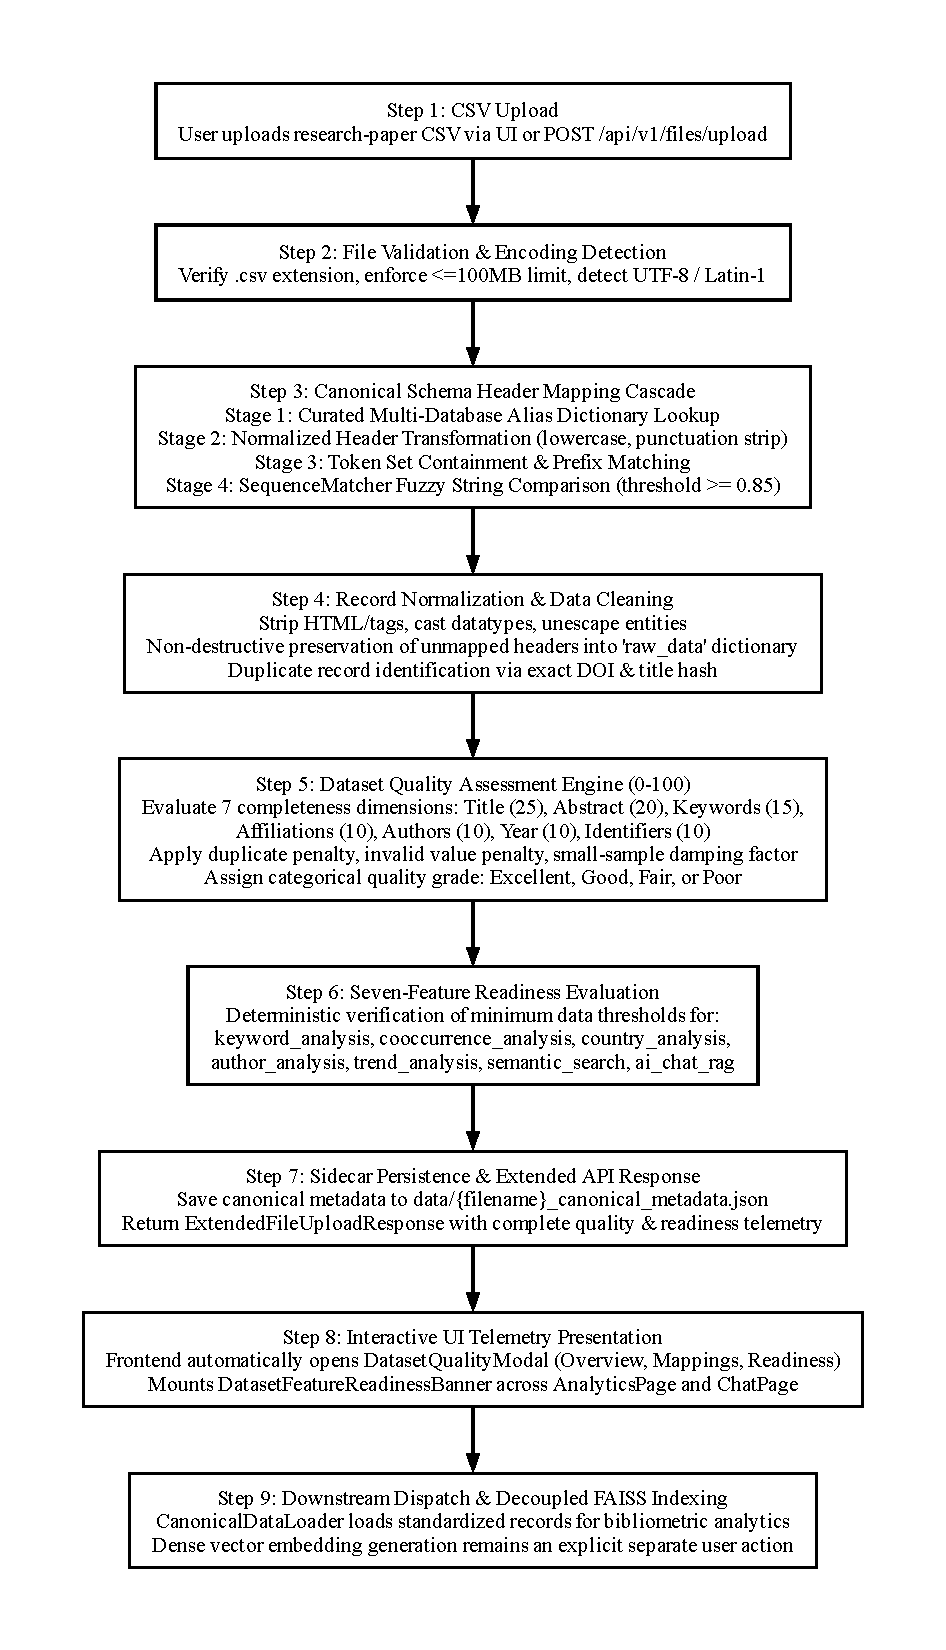
\includegraphics[width=0.92\textwidth]{figures/data_ingestion_workflow.pdf}
\caption{End-to-End Execution Sequence of the Universal Ingestion and Quality Engine}
\label{fig:data_ingestion_workflow}
\end{figure}

Figure~\ref{fig:data_ingestion_workflow} outlines the nine-stage ingestion pipeline executed whenever a user uploads an arbitrary research CSV file.

\subsection{Canonical Dataset Normalizer (dataset\_normalizer.py)}
The normalizer standardizes heterogeneous input schemas into a unified representation.

\subsubsection{The 20-Field Canonical Paper Schema}
The system maps all recognized data fields into a strict 20-field schema:
\begin{enumerate}
    \item \texttt{id}: Unique record identifier (derived from DOI, PMID, or deterministic row hash).
    \item \texttt{title}: Paper title string.
    \item \texttt{abstract}: Comprehensive manuscript abstract.
    \item \texttt{authors}: Delimited string or list of author names.
    \item \texttt{year}: 4-digit publication year (integer).
    \item \texttt{doi}: Digital Object Identifier normalized to standard format (e.g., \texttt{10.xxxx/...}).
    \item \texttt{pmid}: PubMed Unique Identifier.
    \item \texttt{pmcid}: PubMed Central Identifier.
    \item \texttt{journal}: Publishing journal or source venue name.
    \item \texttt{publisher}: Publishing organization.
    \item \texttt{keywords}: Author keywords or extracted key phrases.
    \item \texttt{mesh\_terms}: Medical Subject Headings (MeSH).
    \item \texttt{affiliations}: Author institutional affiliation strings.
    \item \texttt{countries}: Extracted sovereign country names.
    \item \texttt{citation\_count}: Inbound citation metric (integer).
    \item \texttt{reference\_count}: Outbound references count (integer).
    \item \texttt{url}: Primary landing page URL.
    \item \texttt{pdf\_url}: Direct PDF link.
    \item \texttt{source\_database}: Source repository identifier (e.g., \texttt{pubmed}, \texttt{scopus}).
    \item \texttt{raw\_data}: Dictionary preserving all original unmapped columns.
\end{enumerate}

\subsubsection{Four-Stage Header Matching Cascade}
To identify incoming columns without manual user mapping, the normalizer executes a four-tier matching cascade:
\begin{itemize}
    \item \textbf{Stage 1: Curated Alias Dictionary Lookup.} Matches headers against curated dictionaries containing hundreds of real-world aliases from major databases (e.g., matching \texttt{"Abstract (English)"}, \texttt{"AB"}, or \texttt{"Description"} to \texttt{abstract}).
    \item \textbf{Stage 2: Normalized Header Transformation.} Strips non-alphanumeric punctuation, converts text to lowercase, and evaluates canonical equivalence.
    \item \textbf{Stage 3: Token Set Containment.} Tokenizes multi-word headers and identifies canonical targets through token subset analysis.
    \item \textbf{Stage 4: Fuzzy String Matching.} Applies \texttt{difflib.SequenceMatcher} to detect typographical variants, assigning a mapping when string similarity $\ge 0.85$.
\end{itemize}

\subsubsection{Non-Destructive Raw Data Preservation}
No source information is ever discarded. Any column not mapped to the 20 canonical fields is automatically serialized into the \texttt{raw\_data} JSON dictionary for each record. The original uploaded CSV file is preserved intact on disk.

\subsection{Dataset Quality Assessment Engine (dataset\_quality.py)}
The quality engine evaluates dataset hygiene, computing an overall score between 0 and 100.

\subsubsection{Mathematical Quality Scoring Formula}
The base quality score represents a weighted summation of completeness across seven primary metadata dimensions:

\begin{equation}
\label{eq:quality_score}
\text{Base Score} = \sum_{i=1}^{7} W_i \times \text{Coverage}(A_i)
\end{equation}

\noindent where the weights $W_i$ are assigned as:
\begin{itemize}
    \item Title Coverage: 25\%
    \item Abstract Coverage: 20\%
    \item Keywords Coverage: 15\%
    \item Affiliations / Countries Coverage: 10\%
    \item Authors Coverage: 10\%
    \item Publication Year Coverage: 10\%
    \item Identifiers (DOI / PMID) Coverage: 10\%
\end{itemize}

\subsubsection{Deductions, Penalties, and Damping}
The final score applies deductions for duplicates and invalid values, scaled by a small-sample damping factor:

\begin{equation}
\text{Duplicate Penalty} = \min\left(10.0, \frac{\text{Duplicates}}{N} \times 20.0\right)
\end{equation}

\begin{equation}
\text{Invalid Penalty} = \min\left(5.0, \frac{\text{Invalids}}{N \times \text{Fields}} \times 25.0\right)
\end{equation}

\begin{equation}
\text{Damping Factor} = \min\left(1.0, \frac{N}{5.0}\right)
\end{equation}

\begin{equation}
\text{Final Quality Score} = \max\left(0.0, (\text{Base Score} - \text{Duplicate Penalty} - \text{Invalid Penalty}) \times \text{Damping Factor}\right)
\end{equation}

Datasets are categorized into quality grades: \textbf{Excellent} ($\ge 85$), \textbf{Good} ($\ge 70$), \textbf{Fair} ($\ge 50$), and \textbf{Poor} ($< 50$).

\subsection{Feature Readiness Assessment Engine}
Rather than allowing analytical jobs to crash at runtime due to missing data, the engine deterministically computes the operational readiness of all seven platform features.

\begin{figure}[H]
\centering
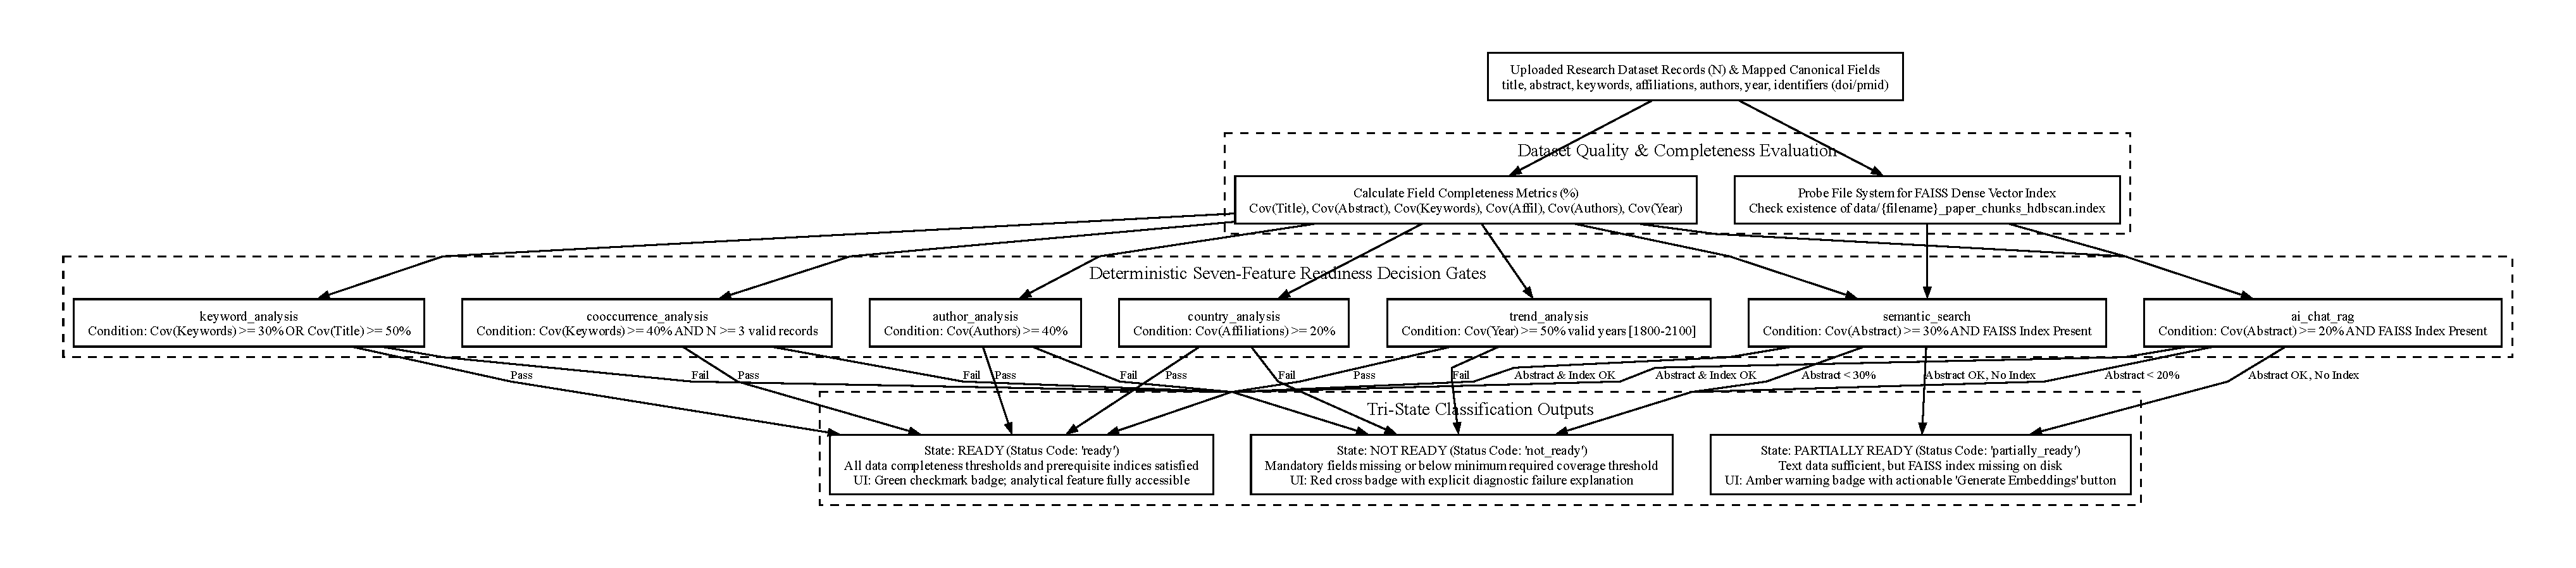
\includegraphics[width=0.92\textwidth]{figures/feature_readiness_workflow.pdf}
\caption{Deterministic Decision Logic of the Seven-Feature Readiness Evaluation Engine}
\label{fig:feature_readiness_workflow}
\end{figure}

As shown in Figure~\ref{fig:feature_readiness_workflow}, each feature is evaluated against specific data availability criteria and classified into one of three distinct operational states:
\begin{itemize}
    \item \textbf{Ready:} Mandatory fields meet or exceed completeness thresholds; feature is fully functional.
    \item \textbf{Partially Ready:} Primary data is available, but prerequisite secondary assets (such as FAISS vector indexes) have not yet been generated.
    \item \textbf{Not Ready:} Mandatory data fields are absent or fall below minimum viable thresholds.
\end{itemize}

Table~\ref{tab:feature_readiness_criteria} enumerates the verified decision criteria across all seven features.

\begin{table}[H]
\centering
\caption{Seven-Feature Readiness Decision Criteria and Thresholds}
\label{tab:feature_readiness_criteria}
\begin{tabularx}{\textwidth}{l X l}
\toprule
\textbf{Feature Identifier} & \textbf{Evaluation Criteria and Minimum Thresholds} & \textbf{Required Fields} \\
\midrule
\texttt{keyword\_analysis} & Keyword coverage $\ge 30\%$ OR Title coverage $\ge 50\%$ & \texttt{keywords}, \texttt{title} \\
\texttt{cooccurrence\_analysis} & Keyword coverage $\ge 40\%$ AND valid records $N \ge 3$ & \texttt{keywords} \\
\texttt{country\_analysis} & Affiliation or country coverage $\ge 20\%$ & \texttt{affiliations}, \texttt{countries} \\
\texttt{author\_analysis} & Author name coverage $\ge 40\%$ & \texttt{authors} \\
\texttt{trend\_analysis} & Valid publication year coverage $\ge 50\%$ (years 1800--2100) & \texttt{year} \\
\texttt{semantic\_search} & Abstract coverage $\ge 30\%$ AND FAISS index present on disk & \texttt{abstract}, FAISS index \\
\texttt{ai\_chat\_rag} & Abstract coverage $\ge 20\%$ AND FAISS index present on disk & \texttt{abstract}, FAISS index \\
\bottomrule
\end{tabularx}
\end{table}

\subsection{Canonical Data Loader (canonical\_loader.py)}
The \texttt{CanonicalDataLoader} class serves as the unified programmatic interface for consuming normalized records. When analytical services invoke:

\begin{lstlisting}[language=python]
df, metadata = CanonicalDataLoader.load_canonical_dataframe(
    filename="uploaded_paper.csv",
    exclude_duplicates=True
)
\end{lstlisting}

\noindent the loader checks for an existing sidecar cache (\texttt{data/uploaded\_paper\_canonical\_metadata.json}). If present, it loads the cached telemetry; if absent, it executes on-the-fly normalization, creates the sidecar cache, and returns a clean, deduplicated Pandas DataFrame. Furthermore, \texttt{apply\_index\_status\_overlay()} dynamically checks disk storage for vector indexes, ensuring that readiness telemetry always reflects real-time file availability.

\subsection{Frontend Telemetry Integration}
The frontend presents this telemetry through two primary components:
\begin{itemize}
    \item \textbf{Dataset Quality Modal (\texttt{DatasetQualityModal.tsx}):} Automatically opens upon CSV upload. Contains three interactive tabs: \textit{Overview} (Overall Score, Grade, Hygiene Metrics), \textit{Column Mappings} (Mapped vs Unmapped Columns, Recognition Confidence), and \textit{Feature Readiness} (Tri-state badges and diagnostic guidance).
    \item \textbf{Dataset Feature Readiness Banner (\texttt{DatasetFeatureReadinessBanner.tsx}):} Persistently mounted at the top of \texttt{AnalyticsPage.tsx} and \texttt{ChatPage.tsx}. Alerts researchers if analytical features are limited by dataset quality or missing embeddings.
\end{itemize}

\noindent \textbf{Decoupled Embedding Architecture:} Uploading a CSV file does \textbf{not} automatically generate dense vector embeddings. Generating embeddings remains an explicit, user-initiated operation via the UI or API. If a dataset has sufficient abstracts but lacks a FAISS index, \texttt{semantic\_search} and \texttt{ai\_chat\_rag} are reported as \textbf{Partially Ready} with an actionable prompt to generate embeddings.
